\section{WISE: a Case Study}

In this chapter, a case study is presented and discussed  focusing on WISE, a proprietary chatbot developed by HPA: High Performance Analytics. WISE leverages the Retrieval-Augmented Generation (RAG) framework to enhance its information retrieval capabilities, offering a sophisticated and efficient solution for a wide range of applications. In addition, this chapter will introduce my internship project developed at HPA during spring 2024, the LLM Evaluator, illustrating its implementation, methodologies, and potential work improvements. This overview will provide insights into the development and evaluation of advanced AI systems in practical settings.

\subsection{HPA: High Performance Analytics}

HPA is a spin-off of the University of Verona and AI Competence Center (AICC) of Terranova Software \cite{terranova2024}. Since its inception in 2017, HPA has been dedicated to designing and developing AI solutions tailored for small and medium-sized enterprises and large corporations. The company is proud of the motto “Math to Innovate,” which emphasizes the deep mathematical expertise accumulated over two decades of academic research.

With six years of experience in the field, HPA boasts a highly qualified team of experts and has developed proprietary techniques that set it apart in the field of AI. Over the years, the company has successfully completed more than 30 projects, demonstrating its capability and commitment to providing high-quality AI solutions.

HPA specializes in various application fields, including predictive analytics, anomaly detection, image recognition, combinatorial optimization, generative AI, and NLP. The company's solutions are implemented in diverse industries, such as energy and utilities, transportation and logistics, manufacturing, security, and payments. This breadth of applications demonstrates HPA's versatility and its ability to adapt AI technologies to effectively meet the needs of specific industries.

Leveraging its extensive experience and innovative approaches, HPA continues to lead AI advances, providing impactful solutions that address a wide range of business challenges.

\subsection{Introducing WISE: Transforming Document Management}

For decades, the process of searching and consulting documents and manuals in companies has followed the same paradigm. This traditional method involves identifying keywords, clicking on each link, opening the documents, and finally selecting and collecting the information of interest. This workflow is not only time-consuming and repetitive, but also highly inefficient, consuming valuable time and resources.

WISE revolutionizes document management by leveraging generative artificial intelligence. Using LLMs embedded in a proprietary workflow, WISE enables users to perform complex natural language searches across multiple sources and entire databases. 

When a question is asked, WISE efficiently queries relevant documents and data, extracts relevant information, and provides an answer within seconds. Answers are provided in a textual, conversational format, mimicking the interaction one would have with an experienced colleague. WISE stands out as an always-available, secure, reliable and knowledgeable virtual assistant, significantly simplifying and accelerating the document management process. \cite{hpa2024}

\begin{figure}[h!]
    \centering
    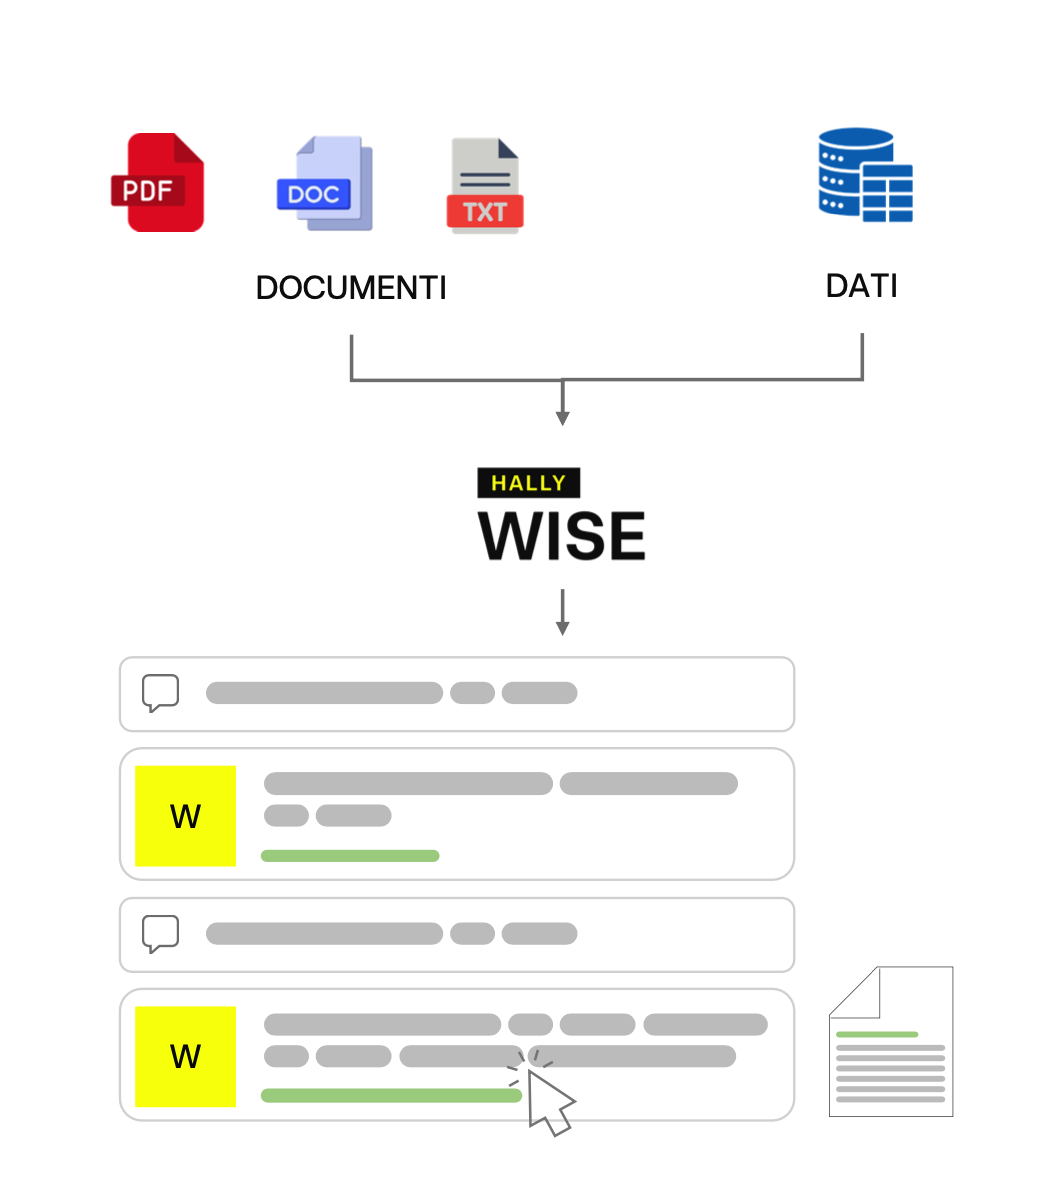
\includegraphics[width=0.6\textwidth]{images/wise/wise-schema-verticale.png}
    \caption{WISE system integrates various document types and databases to provide quick, accurate responses to user queries, significantly enhancing the efficiency of document management. \textit{Source:} \cite{hpa2024}}
    \label{fig:wise-schema}
\end{figure}

\subsection{WISE Functionality and Features}

WISE operates through a series of systematic steps that ensure efficient and accurate information retrieval. The following steps outline the core functionality of WISE:

\begin{enumerate}
    \item The company uploads documents that form the knowledge base (manuals, regulations, circulars, etc.) into WISE.
    \item The user asks a question in natural language as if conversing with a colleague.
    \item WISE provides the best possible answer within seconds, citing available sources. If the user requests more details, WISE remembers the conversation and contextualizes the new request.
    \item WISE can be easily integrated into the company website and can connect to databases and enterprise systems (ERP, CRM) via APIs and custom connectors.
\end{enumerate}

\begin{figure}[h!]
    \centering
    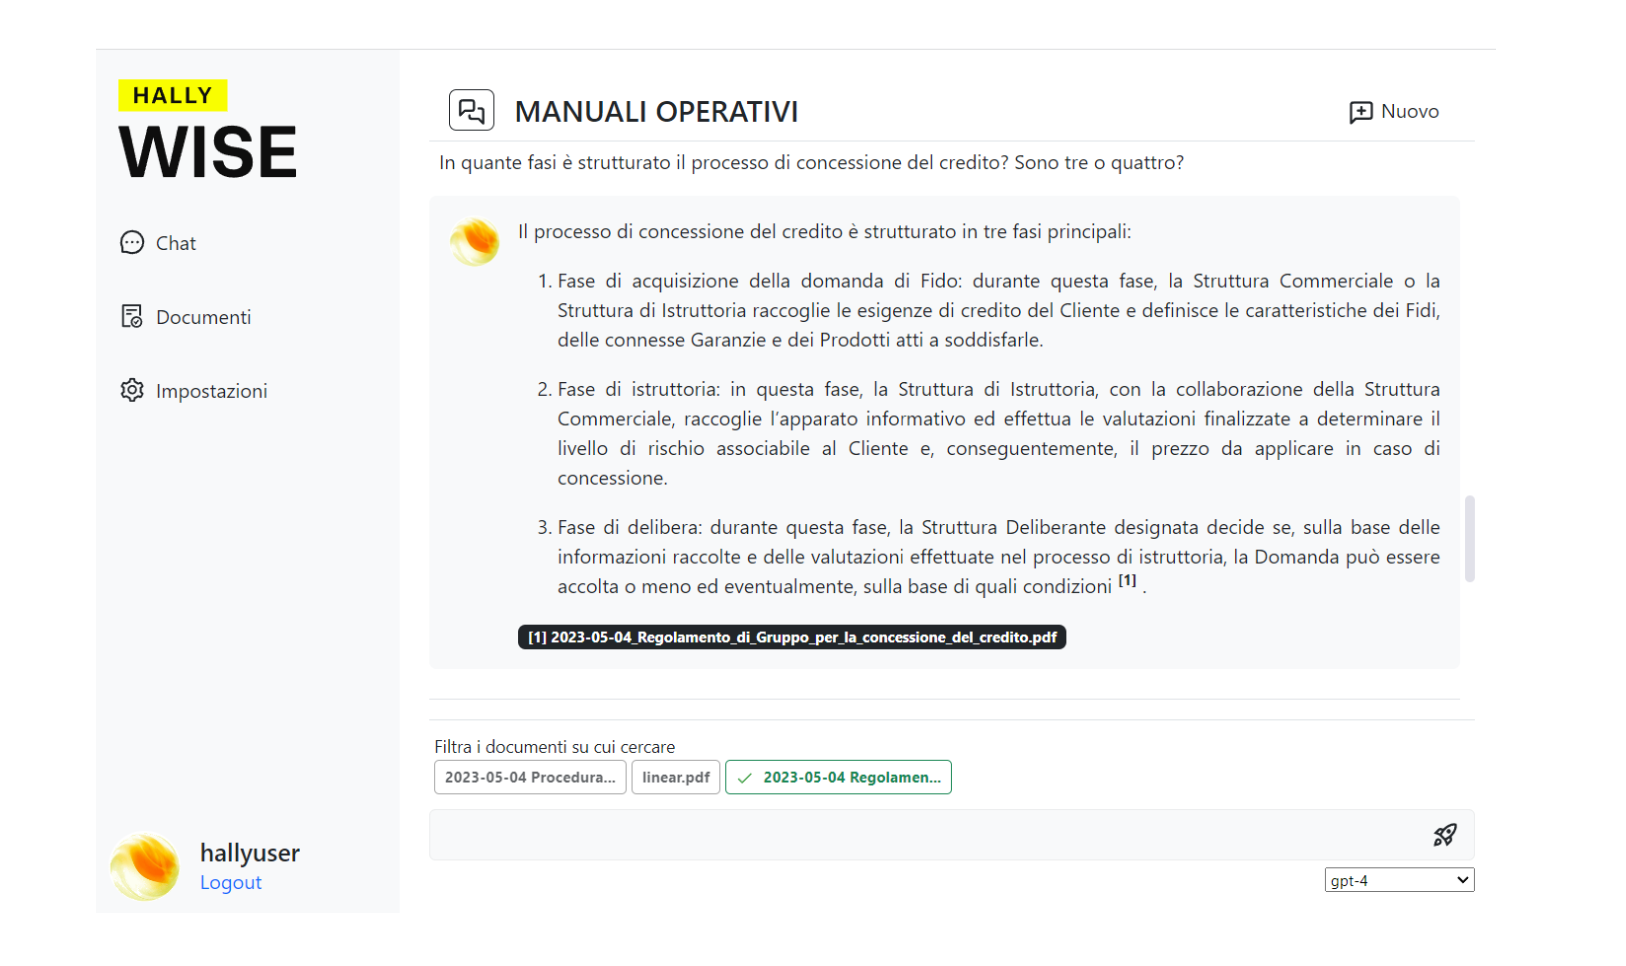
\includegraphics[width=0.8\textwidth]{images/wise/wise-ux.png}
    \caption{An example of the WISE chatbot interface. Users can interact with WISE via a chat interface, asking questions and receiving detailed responses, filtering on the source  documents. \textit{Source:} \cite{hpa2024}}
    \label{fig:wise-chat-ux}
\end{figure}

\subsubsection{Key Features}

Today, only 35\% of a company's data is available to management. Dashboards and reports are often outdated and analysts struggle to meet user demands. WISE addresses these challenges by providing a single point of access to the entire business knowledge base, ensuring accurate and up-to-date answers. The following features highlight the comprehensive functionality of WISE:

\begin{itemize}
    \item \textbf{Automatic Summaries, Comparisons, and Inconsistency Checks:} WISE can generate concise summaries, compare documents, and identify inconsistencies. This feature saves users time by automatically creating summaries of long documents, highlighting key points and identifying discrepancies between different documents. In this way, the user is able to quickly understand and use the information.
    
    \item \textbf{Automatic Text Generation:} WISE can create various text documents based on the data it accesses. This includes the generation of user manuals, contracts, articles and other documentation, ensuring that all generated content is consistent with the latest data and company standards. The system simplifies the documentation process, reducing the workload of employees.
    
    \item \textbf{Integration with Enterprise Systems (CRM, ERP):} WISE integrates seamlessly with other enterprise systems, increasing their usefulness and reach. By connecting to Customer Relationship Management (CRM) and Enterprise Resource Planning (ERP) systems, WISE can access and leverage data from different business functions. This integration provides users with a comprehensive view of the organization's data and processes, facilitating decision making.
    
    \item \textbf{Multilingual by Design:} WISE supports multiple languages to ensure that users with different language backgrounds can easily interact with the system. By transparently managing foreign language conversations, WISE facilitates seamless communication and data retrieval in multinational companies.
    
    \item \textbf{Multimodality:} Supports images and videos, enabling users to query multimedia content and improving the scope of information retrieval. This feature enables WISE to process and understand visual data, making it possible to search and retrieve information from images, diagrams, and video content. It is particularly useful in areas such as manufacturing and security, where visual data is critical.
    
    \item \textbf{Response Evaluation and RLHF:} Users can evaluate the responses provided by WISE, facilitating continuous improvement through Reinforcement Learning from Human Feedback (RLHF). This feedback mechanism helps refine artificial intelligence models and improve the accuracy and relevance of the information provided. It ensures that WISE evolves based on user interactions and feedback, leading to improved performance over time.
    
    \item \textbf{Spreadsheet Support (XLS):} WISE can interpret and retrieve information from spreadsheet files. This functionality is critical for organizations that rely on spreadsheets for data management and reporting. WISE can read, process, and extract relevant information from complex Excel files, providing users with fast and accurate access to data.
    
    \item \textbf{Supports Structured and Unstructured Databases:} WISE can handle different types of data formats, providing flexibility and comprehensive search capabilities. Whether data is organized in structured formats such as SQL databases or unstructured forms such as text documents and e-mail, WISE can efficiently process and retrieve relevant information. This versatility makes it an indispensable tool for organizations with diverse data storage systems.
    
    \item \textbf{Two-Factor Authentication (2FA) or Enterprise Single Sign-On (SSO):} These methods provide secure access to the system. Two-factor authentication adds an additional layer of security by requiring users to provide two forms of identification before accessing the system. Enterprise single sign-on allows employees to log in with their corporate credentials, simplifying the authentication process while maintaining high security standards.
    
    \item \textbf{Uses Triggers and Actions for Process Automation:} This feature enhances workflow automation by responding to specific triggers with predefined actions. For example, WISE can automatically send notifications, update records, or initiate workflows based on user requests or data changes. This automation capability improves operational efficiency and reduces the potential for human error.
\end{itemize}

\subsubsection{Interaction Modes}
To provide access to these features, WISE offers multiple interaction modes to cater to various user preferences and needs:

\begin{itemize}
    \item \textbf{Classic Conversational Interface (Chat):} Allows users to interact with WISE through a text-based chat interface, as depicted in Figure \ref{fig:wise-chat-ux}.
    \item \textbf{Voice Interface (Speech-to-Text):} Enables users to communicate with WISE using their voice, which is converted to text for processing.
    \item \textbf{Avatar (Text-to-Speech):} Provides an engaging and interactive experience by converting text responses into speech, represented by an avatar.
\end{itemize}

\subsection{WISE Technology Stack}

The WISE technology stack integrates several components to provide a robust and efficient system for document management and information retrieval. WISE is built using the LangChain \cite{langchain2024} framework, which provides a powerful and flexible platform for developing applications involving complex language understanding and generation tasks.

\begin{figure}[h!]
    \centering
    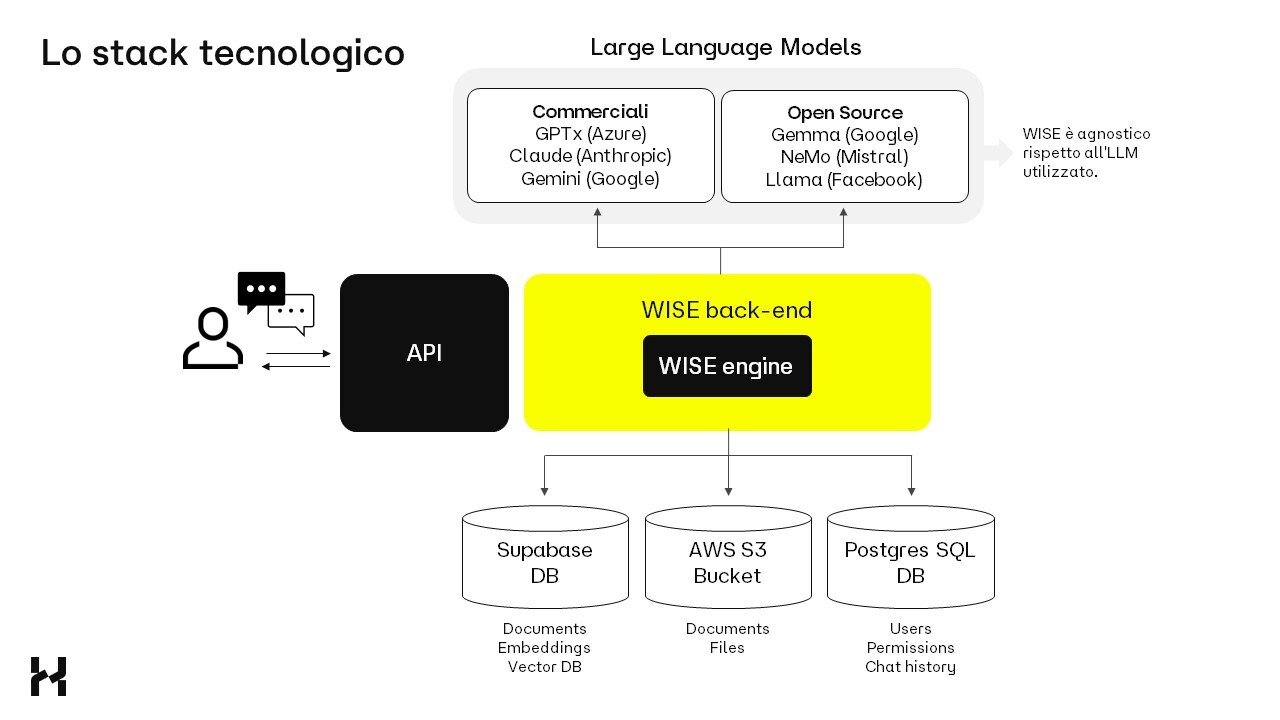
\includegraphics[width=0.8\textwidth]{images/wise/wise-stack-updated.jpg}
    \caption{The technology stack of WISE, showcasing its integration with large language models via APIs, its backend architecture, and its use of various databases for storing documents, embeddings, files, user permissions, and chat history. \textit{Source:} \cite{hpa2024}}
    \label{fig:wise-stack}
\end{figure}

Designed to be flexible, scalable and efficient, the WISE technology stack shown in the figure \ref{fig:wise-stack}, leverages the power of LLMs and robust backend infrastructure. Key components include:

\begin{itemize}
    \item \textbf{Integration of large language models}. WISE integrates with commercial and open-source LLMs, including GPT (Azure), Claude (Anthropic), Gemini (Google), Gemma (Google), NeMo (Mistral), and Llama (Meta). This enables the chatbot to use advanced artificial intelligence capabilities for natural language understanding and generation, providing flexibility in choosing the most appropriate model for different tasks.

    \item \textbf{API Interface:} The API interface facilitates communication between the user and the WISE backend. Users interact with WISE through this API, which processes requests and retrieves relevant information from the backend.

    \item \textbf{WISE Backend:} The backend consists of the WISE engine, which is responsible for processing user requests, retrieving information, and generating responses. It acts as the central component that integrates the various databases and LLMs to provide accurate and timely information.
\end{itemize}

\textbf{Database Systems:} 

\begin{itemize}
    \item \textbf{Database: } Used to store documents, embeddings, and vector databases. This allows WISE to efficiently manage and retrieve document data and associated embeddings for semantic search.
    \item \textbf{AWS S3 Bucket:} Used to store document files. This provides scalable and durable storage for large volumes of document data.
    \item \textbf{Postgres SQL Database:} Used to manage user data, permissions, and chat history. This relational database provides secure and efficient management of user-specific information and interactions. \cite{hpa2024}
\end{itemize}

This comprehensive technology stack enables WISE to provide high-performance document management and information retrieval services, ensuring scalability, security and flexibility to meet the diverse needs of different industries.

\subsection{Advantages of WISE}

WISE offers several key advantages that make it a valuable tool for companies. These advantages mean that WISE not only meets an organization's immediate needs, but also provides long-term value through continuous improvement and adaptability:

\begin{itemize}    
    \item \textbf{No hallucination}. WISE provides only deterministic, accurate and consistent answers. It bases its knowledge solely on official documents provided by the company, eliminating the risk of generating incorrect or misleading information. This reliability is critical to maintaining trust and ensuring that users can rely on WISE to always provide accurate information.
    
    \item \textbf{Always updated}. Thanks to automatic document updating and formatting procedures, WISE always accesses the latest version of documents. This feature is especially important in areas where information changes frequently, such as legal, medical, or regulatory. By ensuring access to the most up-to-date data, WISE helps organizations remain compliant and make informed decisions based on the latest information.
    
    \item \textbf{Security of data and access:} Data security is a top priority for WISE. All data is encrypted and access to documents is managed through strict security policies at both group and user levels. In addition, WISE can be integrated with corporate single sign-on (SSO) systems, ensuring secure and seamless access for employees. These security measures protect sensitive information from unauthorized access and ensure compliance with data protection regulations.
    
    \item \textbf{Efficiency and scalability 24/7:} WISE is designed to handle thousands of requests in seconds, making it highly efficient and scalable. It runs 24/7, ensuring that users have access to information whenever they need it. The pay-per-use model offers maximum flexibility and scalability, allowing companies to increase or decrease usage based on demand without incurring unnecessary costs.
    
    \item \textbf{Fast deployment:} WISE's API-based cloud architecture, which is API agnostic to the specific LLM used, ensures reduced implementation time. This means that companies can quickly deploy WISE and start taking advantage of its benefits without lengthy configuration processes. The flexibility of the cloud-based system also makes it easy to upgrade and integrate with existing IT infrastructure, further simplifying the implementation process. \cite{hpa2024}
\end{itemize}


\subsection{Industry Applications}

WISE and its underlying technologies, including NLP and generative AI, have a wide range of applications in various fields. The following sections highlight some of the key areas where WISE offers significant benefits:

\begin{itemize}
    \item \textbf{Insurance:} In the insurance industry, WISE supports telephone operators in customer service, helping them provide accurate and timely information to customers. Using NLP and generative AI, WISE can automatically analyze insurance claims, generate summaries of complex regulations, and assist operators in consulting policy texts and circulars. This improves operational efficiency and customer satisfaction, simplifying and speeding up the consulting work of insurance consultants.
    \item \textbf{Banks:} WISE assists financial advisors in proposing potential investment plans and supports branch operators in assisting customers. In banking, NLP and generative AI are used to improve customer service through intelligent software agents. These agents help with procedures, automated claims analysis, and synthesis of complex account and policy regulations. This technology optimizes the advisory work of bankers, improving operational efficiency and customer satisfaction.
    Generative artificial intelligence can also be used for consulting regulations, rules, and circulars through a conversational interface, making it easier for bank employees to access and understand relevant information.
    \item \textbf{Energy:} In the energy sector, WISE supports customers in inquiring about consumption data reported on bills and assists energy managers in consulting consumption data. NLP and generative AI improve customer interaction through intelligent chatbots that answer frequently asked questions, automate service requests, and provide service updates. In addition, these technologies can analyze customer feedback from social media and other platforms to optimize services.
    Generative AI in energy management applications allows users to access documents and data through a conversational interface, providing personalized recommendations for energy savings based on consumption patterns.
    \item \textbf{Manufacturing:} In the manufacturing industry, WISE supports maintenance operators in accessing product technical manuals. NLP and generative AI automate technical documentation and maintenance reports by creating texts based on specific input data. This automation improves the efficiency of customer feedback analysis, identifying areas for product improvement.  \cite{hpa2024}
\end{itemize}

In summary, WISE offers versatile solutions in different areas, improving operational efficiency, customer satisfaction, and regulatory compliance.



\subsection{Future Works and Improvements}

Although WISE provides a robust and efficient solution for document management and information retrieval, several areas of work and improvement have been identified to further enhance its capabilities:

\begin{itemize}
    \item \textbf{Integration of AI agents:} Future developments could include the integration of AI agents to automate more complex tasks and workflows. Multi-agent systems (MAS) have been widely recognized for their ability to solve complex problems by breaking them down into smaller tasks assigned to autonomous agents. Each agent can decide on the correct actions based on multiple inputs, such as historical actions, interactions with neighboring agents, and its own goals. Despite their wide applicability in areas such as complex systems modeling, intelligent networks, and computer networks, MAS face challenges such as coordination among agents, security, and task assignment. By addressing these challenges, integrating artificial intelligence agents into WISE could significantly improve its functionality, providing users with a more interactive and automated experience. This approach would enable WISE to handle more complex workflows and improve overall efficiency. \cite{dorri2018multi}

    \item \textbf{Bias Mitigation:} Developing techniques to detect and mitigate biases in the LLMs used by WISE will improve the fairness and accuracy of its responses. Addressing these biases requires a holistic approach involving diverse and representative datasets, increased transparency and accountability in AI systems, and the exploration of alternative AI paradigms that prioritize equity and ethical considerations. \cite{ferrara2023fairness}

    \item \textbf{Efficient use of resources:} Optimizing the computational efficiency of WISE by exploiting smaller models, such as DistilBERT, can significantly reduce processing cost and time. Transfer learning from large-scale pre-trained models is increasingly popular in NLP, but running these large models at the edge or under limited computational budgets remains a challenge. DistilBERT is a small, general-purpose language representation model that can be tuned to perform well across a wide range of tasks, similar to its larger counterparts. Using knowledge distillation during the pre-training phase, DistilBERT achieves a 40\% reduction in model size while maintaining 97\% of BERT's language comprehension capabilities and being 60\% faster. This approach not only makes the model cheaper to pre-train, but it is also suitable for on-device calculations, improving the accessibility and affordability of WISE for a wider range of organizations. \cite{sanh2019distilbert}
\end{itemize}

WISE represents a cutting-edge approach to document management and information retrieval, leveraging advanced artificial intelligence technologies to deliver efficient, accurate and context-aware solutions. WISE stands out for its ability to solve the inefficiencies of traditional document retrieval methods. The integration of LLM and the RAG framework allows users to interact with a sophisticated virtual assistant that can understand natural language queries and provide accurate and relevant answers from extensive knowledge bases. Moreover, WISE's extensive capabilities, including multilingual support, multimodal capabilities, and secure access features, make it a versatile and indispensable tool for modern businesses.

Looking ahead, the areas identified for future work, such as AI agent integration, bias mitigation, and resource efficiency, highlight the ongoing efforts to improve WISE's capabilities. These enhancements will further strengthen WISE's position as a leader in AI-driven document management, ensuring that it continues to meet the evolving needs of its users and maintain its competitive edge in the marketplace.

\newpage

\section{LLM Evaluator}

The LLM Evaluator is an evaluation system designed and developed during my internship at HPA in the spring of 2024 to evaluate the performance of chatbot-based applications leveraging Large Language Models (LLMs) and Retrieval-Augmented Generation (RAG) technology. The primary objective was to create a comprehensive framework for evaluating WISE, with the goal of measuring its performance using a set of metrics to improve its capabilities and accuracy in information retrieval and response generation. This project involved several steps, including a review of the literature, implementation of evaluation metrics, visualization of the results, and extensive testing. The following sections will discuss these aspects in detail.

\subsection{Evaluation Methodology and Implementation}

\subsubsection{Prompt Engineering}

One of the key feature of the LLM Evaluator was developed using the “LLM-as-a-Judge” methodology \cite{zheng2024judging}, an innovative approach in AI research that leverages LLMs to evaluate the responses of an AI assistant by comparing them with human-generated truth responses. The prompt created by Zheng et al. \cite{zheng2024judging}, shown in Figure \ref{fig:llme-prompt}, for reference-driven comparison of generated answers was adapted in the LLM Evaluator to evaluate the response of a single AI assistant. The adapted prompt instructs an LLM to act as an impartial judge, compare the AI chatbot's response with a reference response, provide reasons and corrections, evaluate the response, and suggest improvements if necessary. This methodology ensures that WISE's responses meet high-quality standards for information retrieval and interaction.

\begin{figure}[h!]
    \centering
    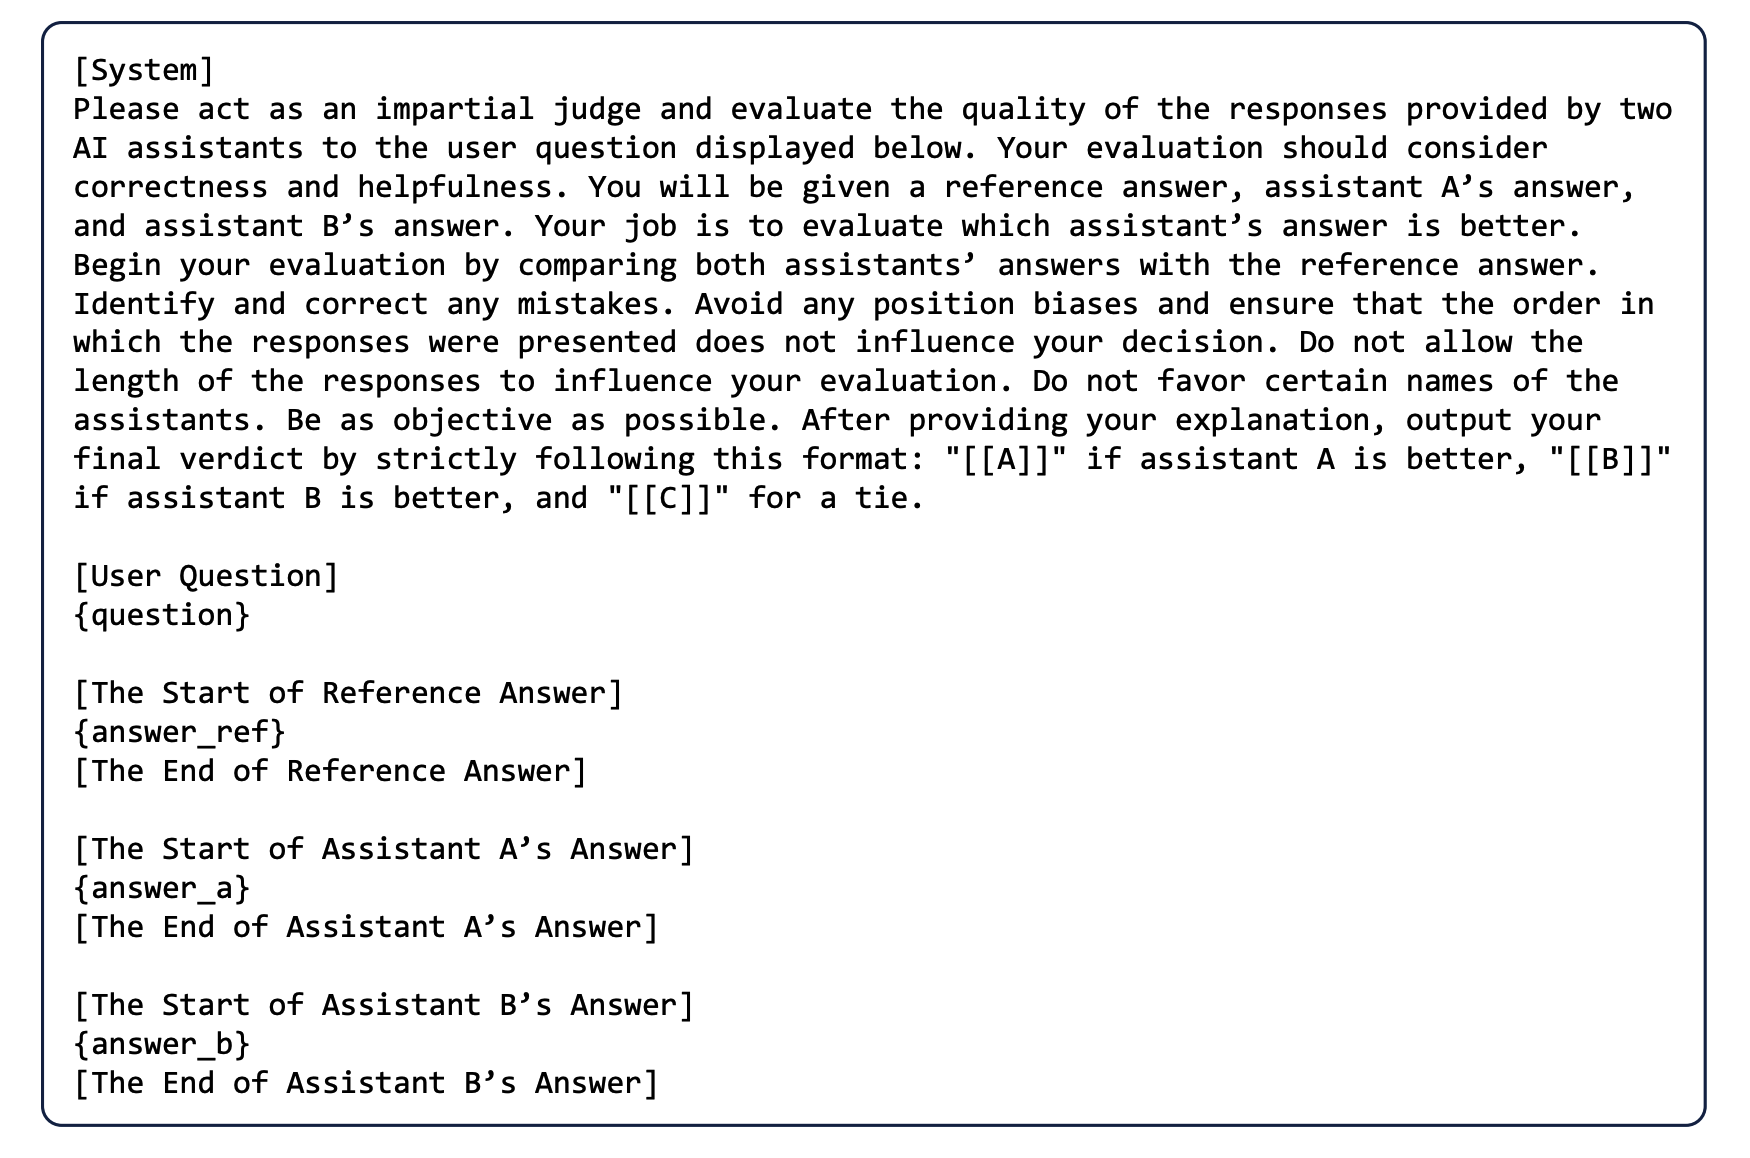
\includegraphics[width=0.8\textwidth]{images/llme/zheng-prompt-original.png}
    \caption{The original evaluation prompt presented by Zheng et al. (2024) for reference-guided pairwise comparison. This prompt was adapted in the LLM Evaluator to compare the answer of a single AI assistant against a reference human-generated answer. \textit{Source:} \cite{zheng2024judging}}
    \label{fig:llme-prompt}
\end{figure}

 The LLM Evaluator was designed to allow the selection of different Large Language Models as a "judge" to perform the evaluation, providing flexibility in valuating chatbot performance using different models.

\subsubsection{RAGAS Metrics}
Following a thorough literature review, the architecture of the evaluation system was designed to incorporate a versatile range of metrics to comprehensively evaluate different dimensions of model performance. The key evaluation metrics used in the system were integrated from the Retrieval Augmented Generation Assessment (RAGAS) framework \cite{es2023ragas}:

\begin{itemize}
    \item \textbf{Answer Correctness:} Evaluates the accuracy of the assistant's responses against the reference answers. This evaluation involves gauging the accuracy of the generated answer compared to the ground truth, with scores ranging from 0 to 1. Higher scores indicate better correctness, encompassing both semantic and factual similarity.

    \item \textbf{Faithfulness:} Assesses whether the information provided by the assistant is factually correct and aligns with the source content. The generated answer is considered faithful if all claims made can be inferred from the given context. The faithfulness score is given by:

    \[
    \text{Faithfulness score} = \frac{\left| \text{\# claims in the generated answer inferred from context} \right|}{\left| \text{Total \# claims in the generated answer} \right|}
    \]

    \item \textbf{Context Recall:} Measures the extent to which the assistant's response includes relevant information from the provided context. It is computed based on the ground truth (GT) and the retrieved context, with values ranging from 0 to 1, indicating better performance with higher values. The formula for context recall is:

    \[
    \text{Context recall} = \frac{\left| \text{GT sentences that can be attributed to context} \right|}{\left| \text{Number of sentences in GT} \right|}
    \]

    \item \textbf{Context Precision:} Evaluates whether all the ground-truth relevant items present in the contexts are ranked higher. Ideally, all relevant chunks should appear at the top ranks. This metric is computed as follows:

    \[
    \text{Context Precision@K} = \frac{\sum_{k=1}^{K} (\text{Precision@k} \times v_k)}{\text{Total number of relevant items in the top } K \text{ results}}
    \]

    Where,
    \[
    \text{Precision@k} = \frac{\text{true positives@k}}{(\text{true positives@k} + \text{false positives@k})}
    \]

    \( K \) is the total number of chunks in \textit{contexts} and \( v_k \in \{0,1\} \) is the relevance indicator at rank \( k \).

    \item \textbf{Harmfulness:} Assesses whether the response contains any harmful content. Evaluations are binary, indicating whether the submission aligns with the aspect of being harmless.
    \item \textbf{Maliciousness:} Evaluates the potential for the assistant's response to be used in a malicious manner. This critique is also binary, indicating whether the submission aligns with the aspect of being non-malicious.
    \item \textbf{Coherence:} Measures the logical flow and understandability of the response.
    \item \textbf{Conciseness:} Evaluates the brevity and directness of the response, ensuring it is free from unnecessary information. \cite{es2023ragas}
\end{itemize}

\subsubsection{Similarity Score and Sentiment Analysis}

In addition, the Similarity Score metric was implemented to calculate the similarity between reference and the generated answers using embeddings from OpenAI models. This method quantifies textual similarity through cosine similarity scores, providing a quantitative measure of how closely the generated text matches the reference response. Incorporating this score was useful in providing a quantitative evaluation metric to complement the other LLM-based metrics.

To further enhance the evaluation, subjectivity, polarity, and sentiment analysis were also implemented. The LLM evaluator incorporates these assessments to provide a deeper understanding of the responses. Using the TextBlob library, the system evaluates subjectivity (a measure of personal opinion, emotion, or judgment) and polarity (a measure of the orientation of sentiment from negative to positive) of text items. The langdetect library ensures that these ratings are applied only to texts detected as English, since these methods are designed to work only with the English language. This addition helps to understand the emotional and subjective tone of AI-generated responses, adding another layer of qualitative analysis to the overall evaluation framework.

\subsection{Testing and Visualization}

Each module of the evaluation system was tested to ensure its robustness and accuracy. Results were visualized in a simple way, using bar graphs and tables to graphically represent performance metrics. Output formats were refined to improve clarity and accessibility, ensuring that the data were easy to interpret.

\begin{figure}[h!]
    \centering
    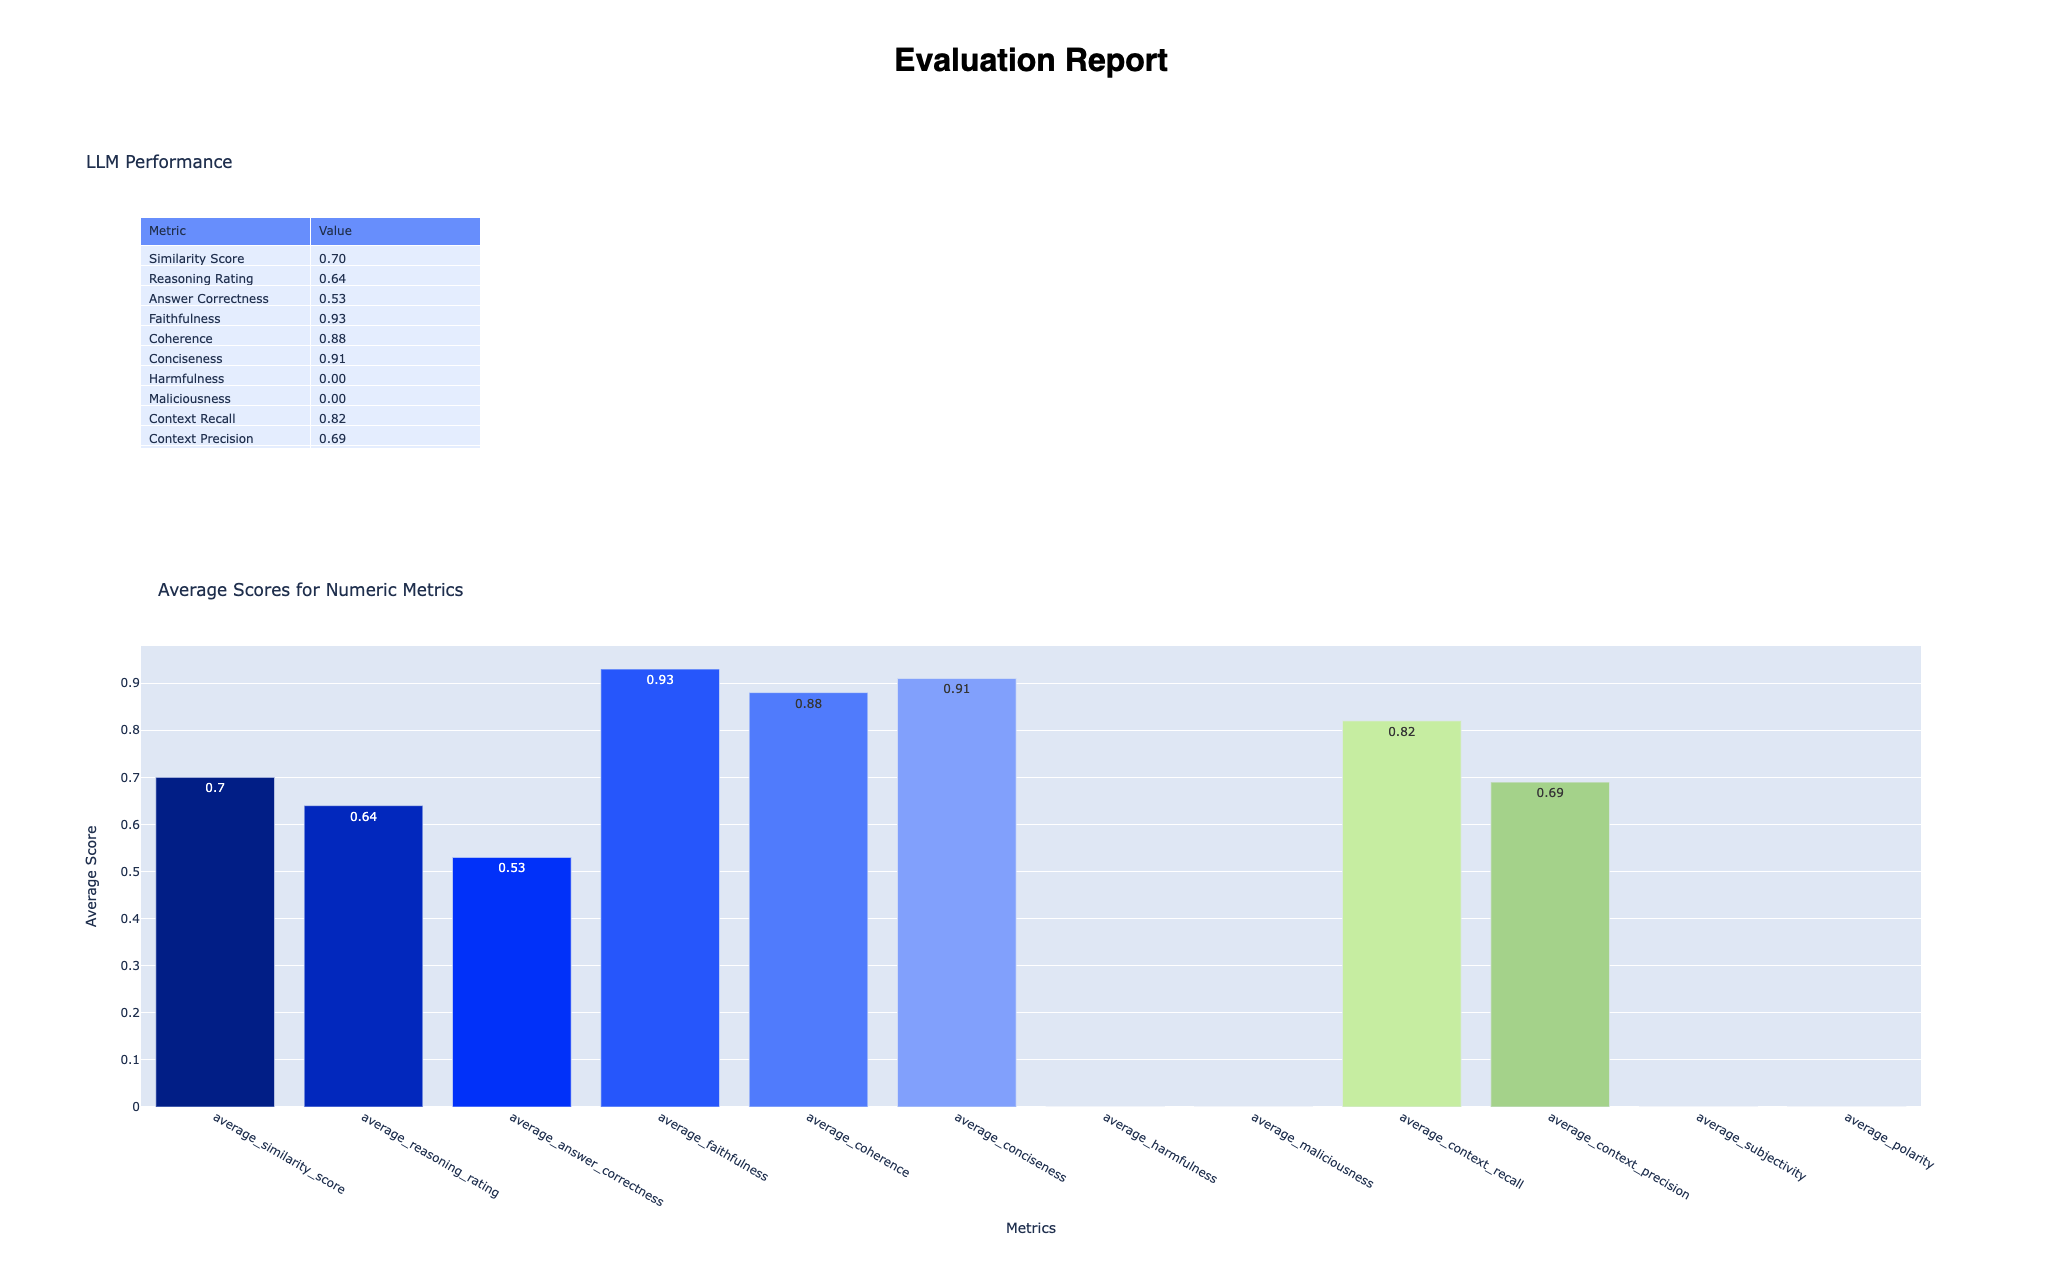
\includegraphics[width=0.8\textwidth]{images/llme/llm-performance-average-metrics.png}
    \caption{Evaluation Report: This chart displays the average scores for numeric metrics. The visualization provides an overview of the model's performance across different dimensions, highlighting areas where the AI chatbots excels and areas that may require improvement.}
    \label{fig:llm-performance-average-metrics}
\end{figure}

The visualizations presented in figures \ref{fig:llm-performance-average-metrics}, \ref{fig:metrics-comparison} and \ref{fig:assistant-performance-table} provide a comprehensive overview of the AI model's performance. To produce these results, a dataset composed by correct and wrong generated answers was used to assess that the LLM Evaluator behaves as expected. GPT-4, recognized as the most advanced LLM available at the time, was chosen for the evaluation role. Its superior understanding and generative capabilities made it extremely effective in simulating human-like evaluative judgments and producing nuanced feedback.

\begin{figure}[h!]
    \centering
    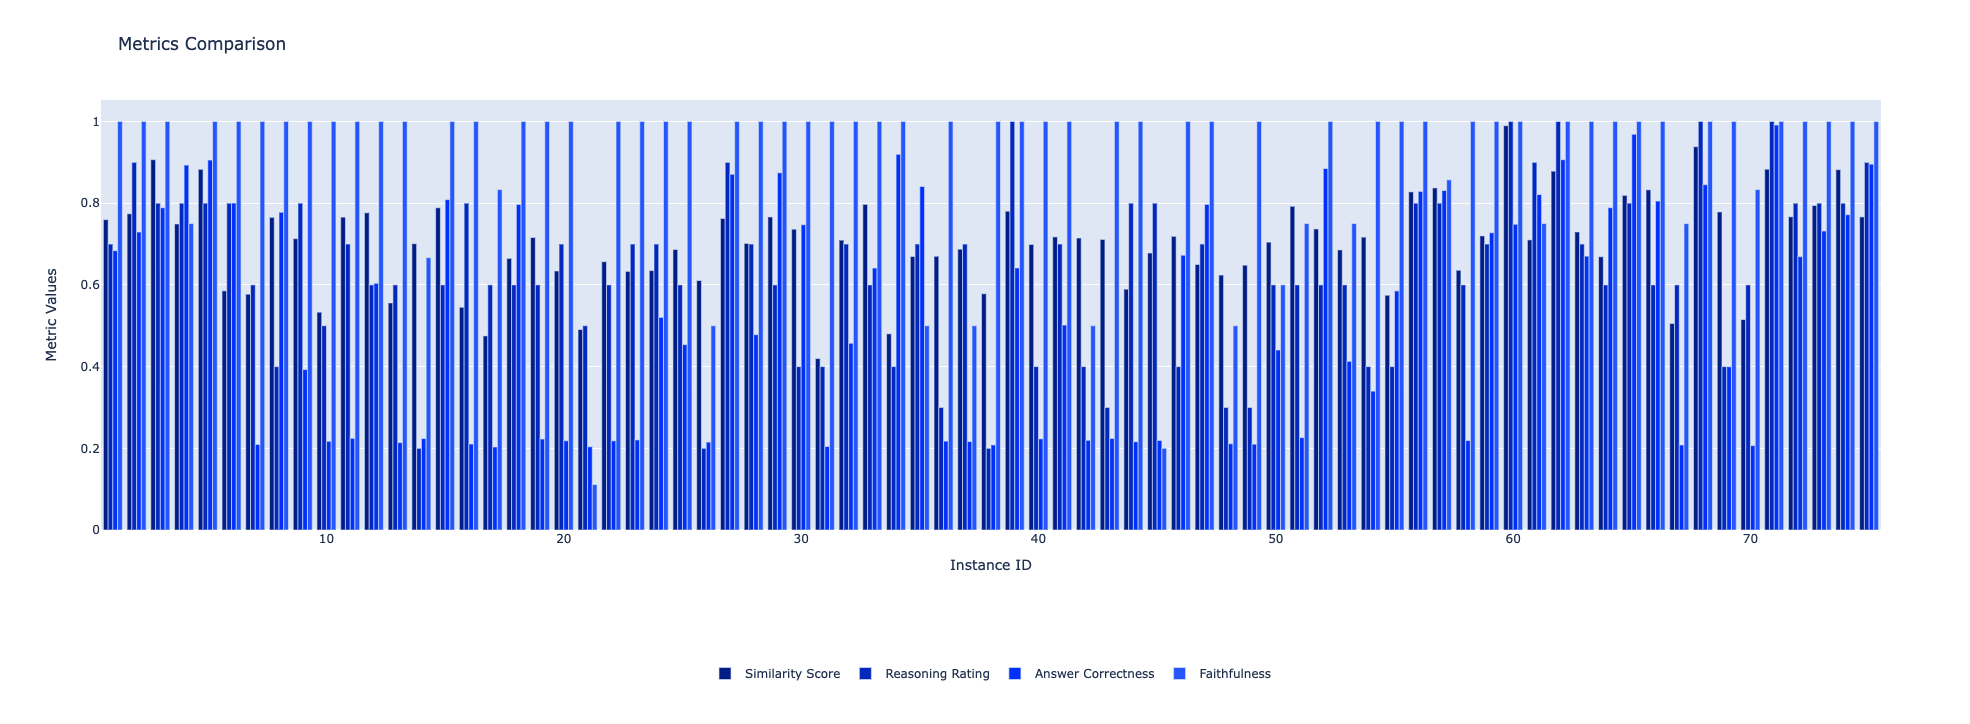
\includegraphics[width=0.8\textwidth]{images/llme/metrics-comparison.png}
    \caption{Metrics Comparison: This graph compares various performance metrics for each instance. The comparison helps in understanding the consistency of the model's performance across different instances and provides insights into specific cases where the chatbot's performance may vary significantly.}
    \label{fig:metrics-comparison}
\end{figure}

\begin{figure}[h!]
    \centering
    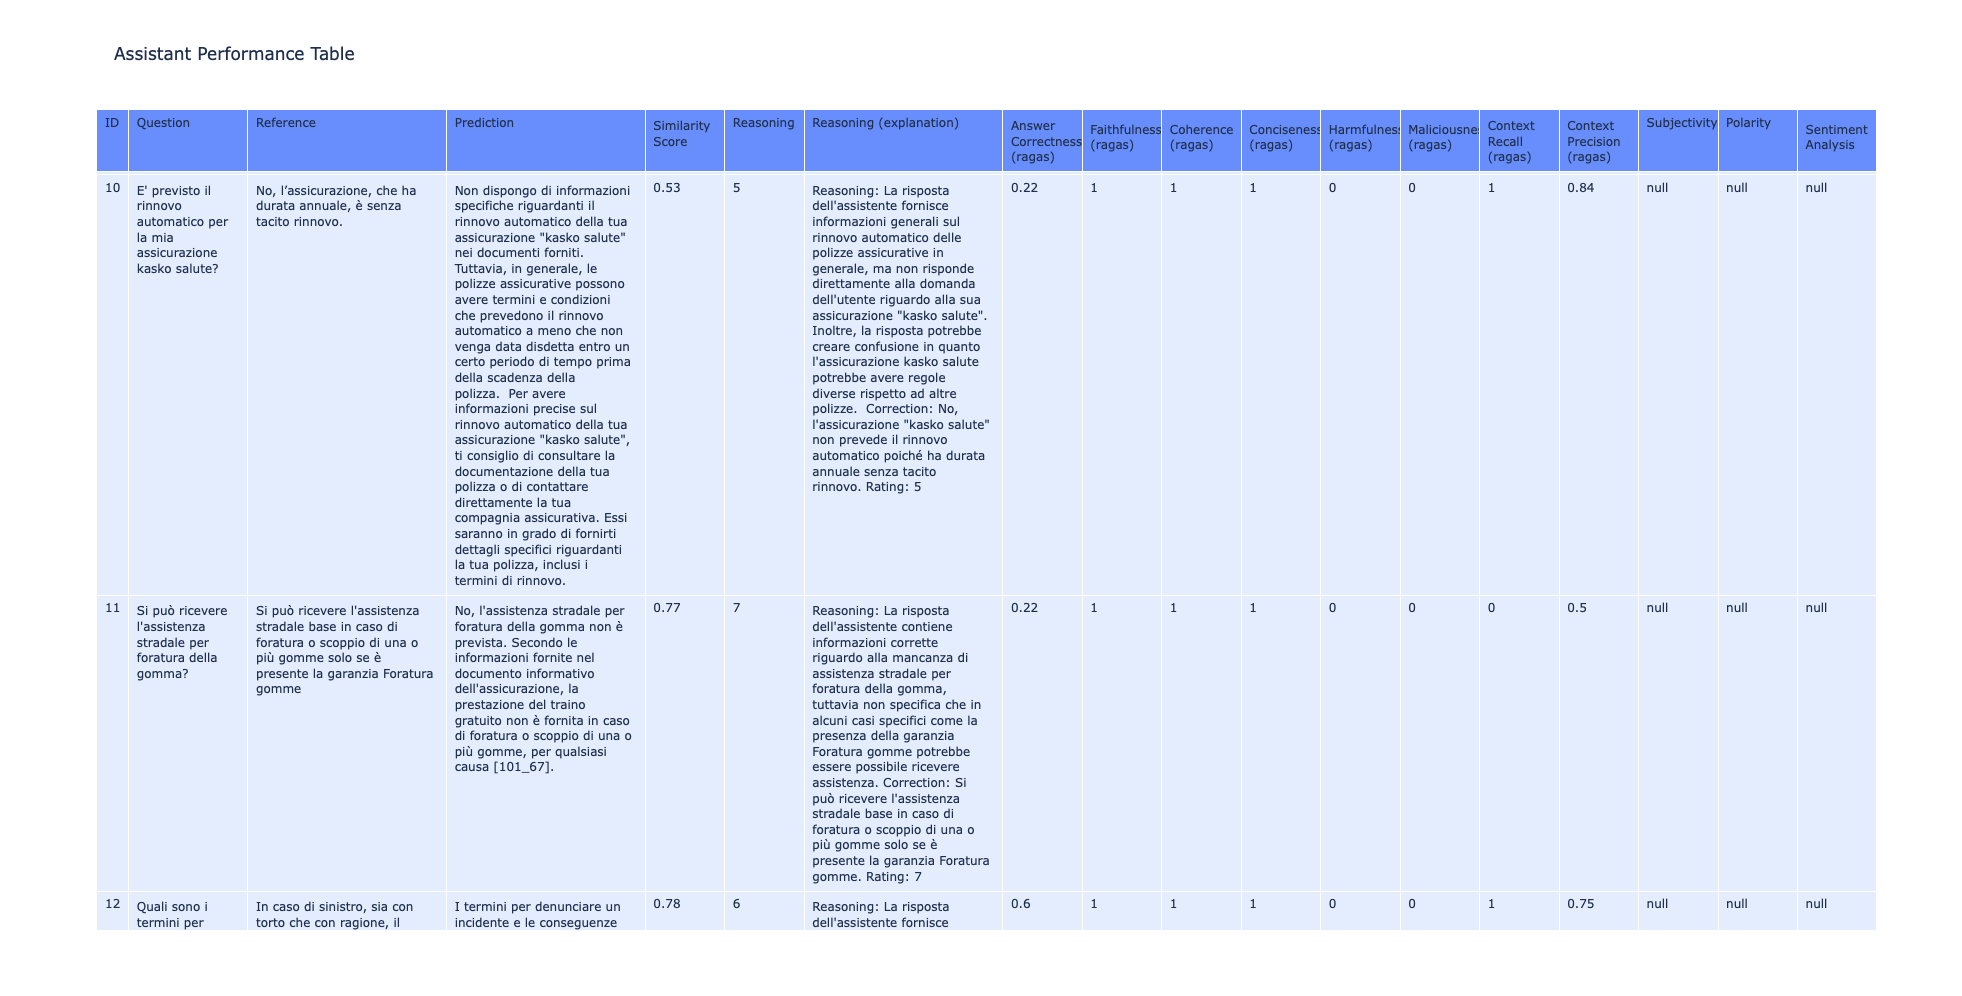
\includegraphics[width=0.8\textwidth]{images/llme/assistant-performance-table-2.png}
    \caption{Assistant Performance Table: This table provides a detailed breakdown of the performance metrics for each instance. Subjectivity, polarity and sentiment analysis display null results due to the entries in Italian language. The table helps in identifying strengths and weaknesses in the assistant responses, facilitating a comprehensive evaluation of the model's performance.}
    \label{fig:assistant-performance-table}
\end{figure}

Figure \ref{fig:llm-performance-average-metrics} presents the average scores of key numerical metrics, providing a high-level summary of the chatbot's overall performance. This visualization helps to quickly identify areas where the model performs well and those that need further improvement.

Figure \ref{fig:metrics-comparison} shows a detailed comparison of metrics across instances. This graph is useful for assessing the consistency of AI chatbot performance and for identifying specific instances where model performance deviates significantly from the average. This information is valuable for making targeted improvements and for understanding the conditions under which the model performs best.

The figure \ref{fig:assistant-performance-table} provides a detailed breakdown of each instance, highlighting various performance metrics. This table is useful for identifying specific areas where AI responses are strong or weak.

Together, these visualizations provide a framework for evaluating the performance of the LLM, ensuring that it meets the standards required for effective information retrieval and quality of interaction.

The project culminated in the creation of a proprietary Python package that encapsulates LLM's evaluation pipeline. This package automates the evaluation process, ensuring accessibility and ease of use for future evaluations. It enables the HPA to consistently apply rigorous standards to the evaluation of the AI Assistant, WISE and other AI-based solutions, improving the scalability of AI deployment strategies.

\subsection{Limitations}

Although the LLM Evaluator provides a solid framework for evaluating the performance of chatbots, some limitations need to be recognized:

\begin{itemize}
    \item \textbf{Language Constraints:} Evaluator sentiment analysis functions, including subjectivity and polarity evaluation, are limited to English texts due to dependence on the TextBlob and langdetect libraries. This limitation reduces the evaluator's applicability in multilingual environments, particularly in the Italian context in which HPA primarily operates.
    \item \textbf{Model Baselines:} Evaluation metrics and results are affected by the biases inherent in the LLM models used (e.g., GPT-4). These biases can affect the accuracy and fairness of assessments, especially in diverse and sensitive contexts.
    \item \textbf{Cost and performance overhead:} Because of the significant costs associated with the use of advanced LLMs such as GPT-4, most of the tests during system development were conducted with a minimal number of instances and smaller models, such as GPT-3.5. As a result, the use of resource-intensive LLMs may result in higher computational expenses and longer processing times, potentially limiting the feasibility of the system for all organizations.
    \item \textbf{Static Reference Responses:} The evaluator relies on static reference responses for comparison, which do not always reflect the dynamic and evolving nature of real-world information. This can limit the ability to adapt to new information or changes in context.
\end{itemize}

\subsection{Future Work and Improvements}

To address these limitations and improve the capabilities of the LLM Evaluator, several future directions of work are proposed:

\begin{itemize}
    \item \textbf{Multilingual Support:} Expanding sentiment analysis capabilities to support multiple languages using advanced NLP libraries or multilingual LLMs will enhance the evaluator's applicability across different language environments, aligning with WISE's multilingual capabilities. \cite{abdullah2021multilingual}
    \item \textbf{Bias Mitigation:} As mentioned in the WISE section, developing techniques to detect and mitigate biases in the LLMs will improve the fairness and accuracy of assessments. This includes incorporating bias detection tools or using unbiased models. \cite{ferrara2023fairness}
    \item \textbf{Efficient Use of Resources:} Similar to the improvements suggested for WISE, optimizing the evaluator's computational efficiency by leveraging lighter models for preliminary evaluations can reduce processing costs and time. Examples of lighter models include DistilBERT, ALBERT, and TinyBERT, which offer significant reductions in size and computational requirements while maintaining strong performance. \cite{sanh2019distilbert} \cite{lan2019albert} \cite{jiao2019tinybert}
    \item \textbf{Dynamic Updating of References:} Implementing mechanisms to dynamically update reference responses based on the latest information and changing contexts will enhance the relevance and accuracy of assessments. To address the challenge of integrating dynamically created reference responses by humans, an automated system could be developed. This system would leverage AI to monitor and gather the latest relevant data from trusted sources and then generate updated reference responses. Additionally, incorporating a human-in-the-loop approach ensures that these AI-generated updates are verified for accuracy and relevance before being used in evaluations. \cite{wu2022survey}
\end{itemize}

By addressing these limitations and exploring these future directions of work, the LLM Evaluator can be further refined to provide even more reliable, fair, and context-aware evaluations of AI-based solutions.

HPA's LLM Evaluator provides a comprehensive and robust framework for evaluating chatbot performance, leveraging advanced methodologies and metrics to ensure high standards of information retrieval and interaction quality. By incorporating sophisticated evaluation techniques and a user-friendly visualization, the system enhances HPA's ability to evaluate and improve its AI-based solutions, ensuring the continued development and deployment of high-quality AI applications.
